\section{Introduction}
\label{sec:intro}

%% introduce Rt 
The effective reproduction number (also called the instantaneous reproduction
number) is a key quantity for understanding infectious disease dynamics including
the potential size of a pandemic, the required stringency of prevention measures,
and the efficacy of other controls. 
The effective reproduction number is defined to be the average number of
secondary infections caused by a new primary infection that occurs at a specific
time. Tracking the time series of this quantity
is therefore useful for understanding whether or not future infections are
likely to increase or decrease from the current state.
Let $\calR(t)$ denote the effective reproduction number at time $t$. Practically,
as long as $\calR(t) < 1$, infections will decline gradually, eventually
resulting in a disease-free equilibrium, whereas when $\calR(t)
> 1$, infections will continue to increase, resulting in endemic
equilibrium. 
%
%% significance/necessity of modeling Rt: 
While $\calR(t)$ is fundamentally a continuous time quantity, it can be related
to data only at discrete points in time $t = 1,\ldots,n$.
This sequence of effective reproduction numbers over time is not observable, but
nonetheless is easily interpretable and retrospectively describes the course of
an epidemic. Therefore, a number of procedures exist to estimate $\calR_t$ from
different types of observed incidence data such as cases, deaths, or
hospitalizations while relying on various domain-specific assumptions.
%% properties: accurate and robust to violation of assumptions 
Importangly, accurate estimation of effective reproduction numbers relies
heavily on the quality of the available data, and, due to the limitations of
data collection, such as underreporting and lack of standardization,
epidemiological models, estimation methodologies rely on various assumptions to
compensate. Because model assumptions may not be easily verifiable from data
alone, it is also critical for any estimation procedure to be robust to model
misspecification. 
%% usage: retrospective or real-time estimation, and prediction

%% literature review: Bayesian approaches: EpiEstim, EpiFilter, EpiNow2, EpiNowCast
Many existing approaches for effective reproduction number estimation are
Bayesian: they estimate the posterior distribution of $\calR_t$ conditional on
the observations. One of the first such approaches is the software \EpiEstim\
\citep{cori2020package}, described by \citet{cori2013new}. This method is
prospective, in that it uses only information available at time $t$ in order to
estimate $\calR_t$ for $i = 1,\ldots, t$. An advantage of \EpiEstim\ is its
straightforward statistical model: incidence data follows the Poisson
distribution conditional on past incidence and $\calR_t$, the conjugate prior
distribution for $\calR_t$ is Gamma with fixed hyperparameters, and the serial
interval distribution is fixed and known. For this reason, \EpiEstim\ requires
little domain expertise for use, and it is computationally fast. \
\citet{thompson2019improved} modified this method to distinguish imported cases from local transmission and
simultaneously estimate the serial interval distribution.
\citet{nash2023estimating} further extended \EpiEstim\ by using
``reconstructed'' daily incidence data to handle cases when the data is not
regularly spaced.
% bayEstim is a version of implementation of {cori2013new} and {thompson2019improved}. 
% 
\cite{abbott2020estimating} proposed a Bayesian latent variable framework,
\texttt{EpiNow2} \citep{EpiNow2}, which leverages incident cases, deaths or
other available streams simultaneously along with allowing additional delay
distributions (incubation period and onset to report delay) in modelling.  
\citet{lison2023generative} proposed an extension that handles missing data by
imputation followed by a truncation adjustment. 
%
\citet{parag2021improved} also proposed a Bayesian approach, \texttt{EpiFilter}
based the (discretized) on Kalman Filter and Smoother. \texttt{EpiFilter} also
estimates the posterior of $\calR_t$ given a Gamma prior and Poisson distributed
incident cases. Compared to \EpiEstim, \texttt{EpiFilter} estimates $\calR_t$
retrospectively using all available incidence data both prior and subsequent to
time $t$, and provides robust estimation in low incidence cases.  
%koyama2021estimating: devised a state-space method for fitting a discrete-time variant of the Hawkes process to a given dataset of daily
\citet{gressani2022epilps} proposed a Bayesian P-splines approach, \EpiLPS, that
assumes negative Binomial distributed incidences. \citet{trevisin2023spatially}
proposed a Bayesian model based on particle filtering to estimate spatially
explicit effective reproduction numbers.
%
Bayesian approaches estimate the posterior distribution of the effective
reproduction numbers, and possess the advantage that the credible intervals can
be easily computed. A limitation of many Bayesian approaches is that they
usually require heavy computational workload, especially when observed data
sequences are long or hierarchical structures are complex.  Below, we compare
our method to two computationally efficient Bayesian models, EpiEstim and
EpiLPS. 

There are also frequentist approaches for $\calR_t$ estimation.
\citet{abry2020spatial} proposed to regularize the smoothness of $\calR_t$
regarding its temporal and spatial evolution. They considered a penalized
regression with a second-order temporal regularization and a spatial
regularization on $\calR_t$ and with Poisson loss. \citet{pascal2022nonsmooth}
extended this procedure by introducing another penalty on outliers for robustness in.  
%
\cite{pircal2023spline} is a spline-based model relying on the assumption of exponential-family distributed incidences. %but in a more continuous-time setting. [Important!] 
\cite{ho2023accounting} estimates $\calR_t$ while monitoring the time-varying
level of overdispersion. 
%
There are other spline-based approaches such as
\cite{azmon2014estimation,gressani2021approximate,pircalabelu2023spline},
autoregressive models with random effects \citep{jin2023epimix} that are robust
to low incidence cases, and generalized autoregressive moving average (GARMA)
model \citep{hettinger2023estimating} that are robust to measurement errors in
incidence data. 
%\cite{jin2023epimix} proposed EpiMix, which included exogenous factors other than incidence cases, and introduced random effects in regression model. It is also robust against low incidence cases. 
%
%There are many other practical considerations in effective reproduction number estimation. \cite{hettinger2023estimating} proposed a generalized autoregresive moving average (GARMA) model, which solved the bias introduced by practical concerns such as particular forms of measurement errors in incidence data. They also incorporates multiple serial interval distributions. %Basically extended EpiEstim. 
%and compartmental models. 


%%%%%%%%%%%%%%%%%%%%%%%%%%%%%%%%%%%%%%%%%% our approach %%%%%%%%%%%%%%%%%%%%%%%%%%%%%%%%%%%%%%%%%%
We propose a retrospective effective reproduction number estimator
called \RtEstim that requires only incidence data. Our model makes the
conditional Poisson assumption, similar to much of the prior work described
above, but is empirically more robust to misspecification. This estimator is a
convex optimization problem with Poisson loss and $\ell_1$ penalty on the
temporal evolution of $\log(\calR_t)$ to impose smoothness over time. 
% , which is known as the trend filtering
% penalty \citep{kim2009ell_1,tibshirani2014adaptive,sadhanala2022exponential}.
% Thus, \RtEstim\ is a \textit{Poisson trend filtering} problem.
% \cite{sadhanala2022exponential} proposed trend filtering with exponential family
% loss on lattices. Here, we focus on Poisson loss on univariate data that is
% modified to integrate the serial interval functions. 
As a result \RtEstim\ generates discrete splines, and the estimated curves
appear to be piecewise polynomials of an order selected by the user.
Importantly, The estimates are locally adaptive, meaning that different time
ranges may posses heterogeneous smoothness.

\begin{figure}[tb]
    \centering
    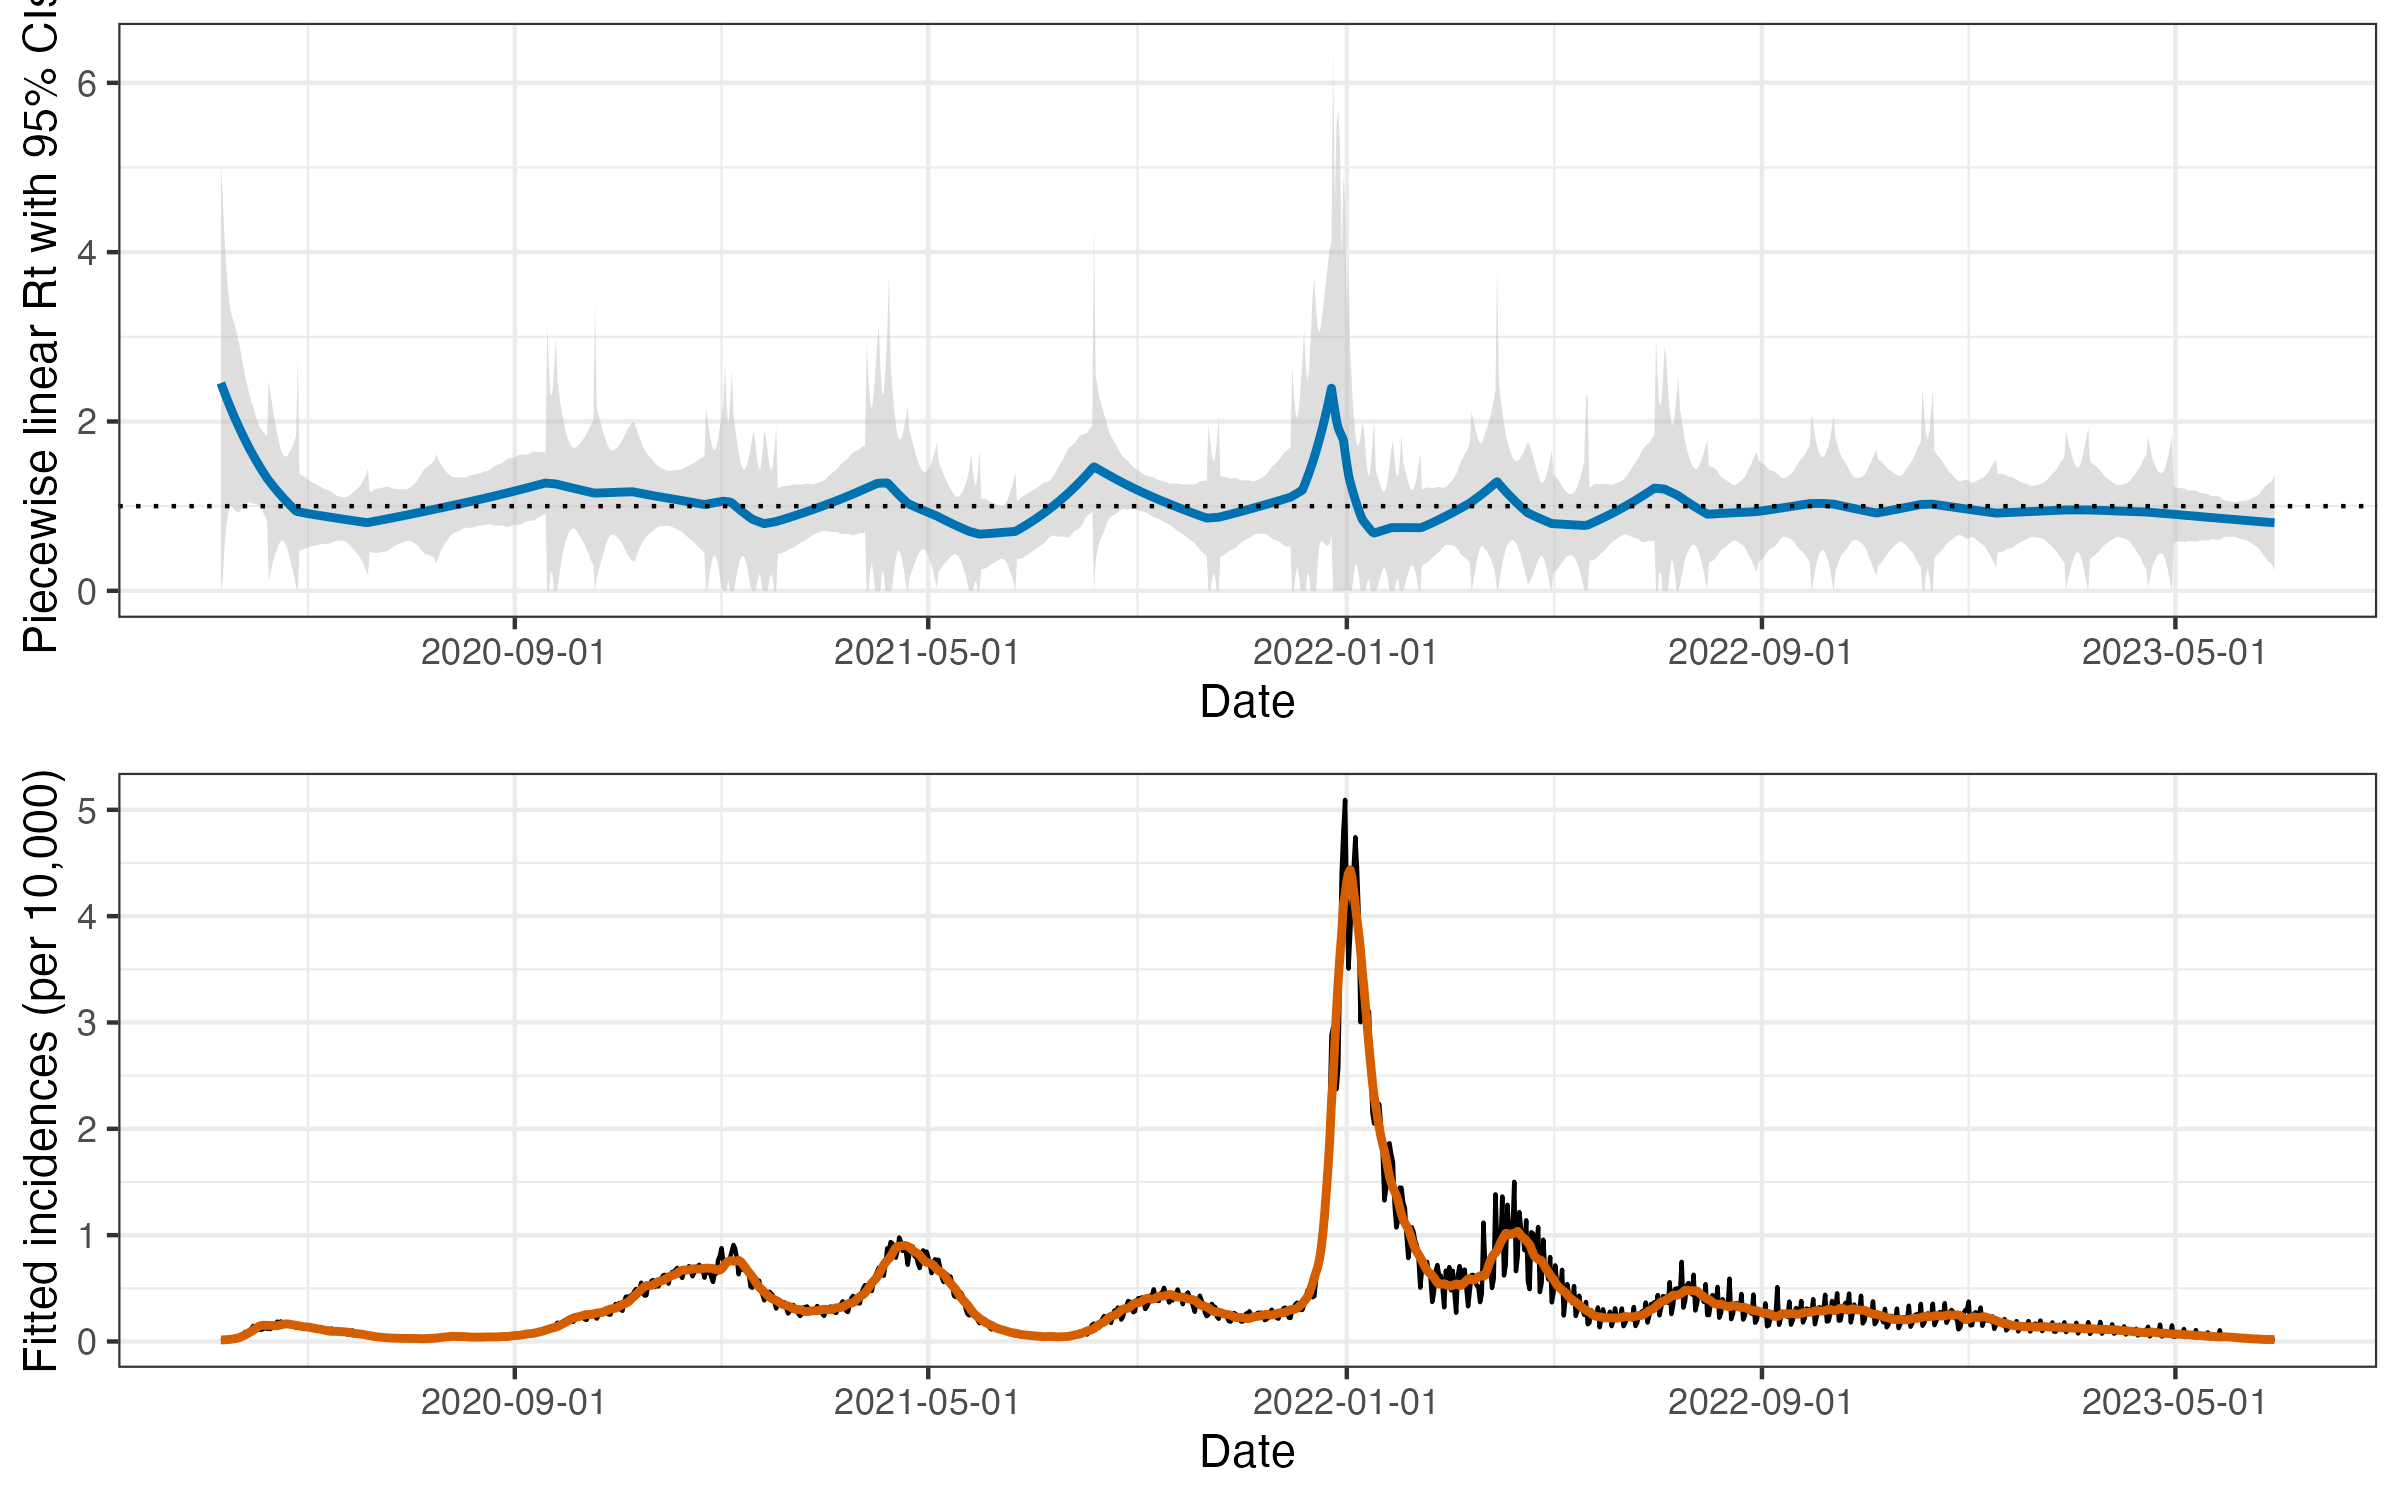
\includegraphics[width=.99\textwidth]{fig/intro-fig.png}
    \caption{A demonstration of effective reproduction number estimation 
    by \RtEstim\ and the corresponding fitted incidence cases for the Covid-19 epidemic 
    in British Columbia, Canada during a period from March 13, 2020 to June 28, 2023. 
    The \textcolor{customblue}{\textbf{blue}} curve in the top panel is the estimated piecewise-linear $\calR_t$ and the 
    gray ribbon is the corresponding 95\% confidence bands. 
    The black curve in the bottom panel is the observed Covid-19 daily confirmed 
    cases, and the \textcolor{customorange}{\textbf{orange}} curve is the fitted incidences corresponding to the 
    estimated $\calR_t$.}
    \label{fig:intro-fig}
\end{figure}

% Due to the limitations including but not limited to
% insufficient surveillance resources and incomplete reporting, the incidence
% cases are only observed to a certain proportion of the unknown, true values.
% Here, we assume that this proportion is smoothly time-varying, which will not
% cause an immediate changing point in the pattern of transmissibility of
% epidemics. With this assumption, we argue that the observable incidences contain
% the true curvature and changing points of the underlying effective reproduction
% numbers of epidemics. We consider a fixed serial interval distribution that
% needs to be pre-specified. It can either be chosen parameters of Gamma
% distribution or a series of probabilities provided by related methods with sum
% $1$. Serial intervals have been studied for specific infectious diseases, such
% as H1N1 influenza and Covid-19, by numerous existing studies
% \citep{white2009estimation,boelle2011transmission,rai2021estimates,alene2021serial,griffin2020rapid}. 
Our approach is straightforward and requires little expertise in domain
knowledge for implementation. 
% \RtEstim\ produces accurate estimations that are empirically robust in model misspecification, i.e., the violation of distributional assumption of incidences. 
% 
 %We follow the common assumption of Poisson distributed incidence data, but the empirical study shows that the estimators are robust in negative binomial settings. 
%Thus, RtEstim is accurate, robust in model misspecification, and computationally efficient. 
% the approach we focus 
We use a proximal Newton method to solve the convex optimization problem along
with a number of computational tricks to produce estimates efficiently,
typically in a matter of seconds even for long sequences of data.
%  Our approach takes the advantage of convex optimization and is
% solved by
% Newton's method, which is known to converge rapidly. %We provide a more
% computationally efficient algorithm for the lowest-degree problem, where
% iterative algorithms can be avoided. 
% Moreover, the sparse structure of the divided difference matrix used in the trend filtering penalty allows further efficiency in computation. 
%Temporal evolution of reproduction numbers considers the progression of reproduction numbers that occurs over time through different temporal intervals. 
In a number of simulated experiments, we show empirically that our approach is
more accurate than existing methods at estimating the true effective reproduction numbers. 

%%%%%%%%%%%%%%%%%%%%%%%%%%%%%%%%%%%%%%%%%% overview %%%%%%%%%%%%%%%%%%%%%%%%%%%%%%%%%%%%%%%%%%
The manuscript unfolds as follows. We first introduce the methodology of
\RtEstim\ including the usage of renewal equation, the development of Poisson
trend filtering estimator, and the proximal Newton algorithm. We explain how 
this method can be interpreted from Bayesian perspective, connecting it to
previous work in this context. We provide illustrative
experiments comparing our estimator to \EpiEstim\ and \EpiLPS. We
then apply our \RtEstim\ on the Covid-19 pandemic incidence in British Columbia
and the 1918 influenza pandemic in the United States. Finally, we conclude with
a discussion on the advantages and limitations of our approach and as well as
describe practical considerations for
the effective reproduction number estimation.
